\section{Methods}
% Intro of three methods
The performance of our layer extraction method is assessed by means of three experiments. \change{First, a model cortex with six layers was constructed. The model cortex has physiologically acceptable folding parameters and its layering satisfies equivolume conditions.}{First, we test the principles of the method on a simulated cortex. The model cortex has physiologically acceptable folding parameters and its layering satisfies equivolume conditions. An OLS estimation is used, as there is no (un)correlated noise added to the system.} \change{Secondly, a high-resolution post-mortem sample of the primary visual cortex (V1) was delineated and the cortical profiles were extracted. As V1 shows a particularly strong layer structure, due to the highly myelinated layer IVc (stripe of Gennari), this structure served as a benchmark for testing our method.}{Secondly, to get a detailed understanding of the behaviour of the spatial GLM with a high number of layers, we used high resolution (post mortem) data from the primary visual cortex (V1). V1 shows a particularly strong layer structure due to the highly myelinated layer IVc (stripe of Gennari), such that the comparative performance of the methods could be easily evaluated.}\change{Thirdly, the method was tested on anatomical data using 11 in-vivo data sets to obtain the cortical profile from V1.}{Thirdly, as the method is likely to be used on human in vivo data, we subsequently assessed anatomical profiles for 11 subjects. We give a detailed account of the influence of the extracted number of layers and we investigate the performance of different FWHMs that can be used for a GLS estimation.} All layerings were performed on upsampled data of twice the resolution. As previously described, the best-case scenarios of the other two methods can be easily characterised in the same theoretical framework as our proposed method. Hence, in order to make the cleanest comparison between methods, all extraction methods start from the same layer volume distribution. 
\begin{itemize}
\item The GLM method: The layer volume distribution is used as design matrix and regressed against the voxel signals.
\item The interpolation method: the same design is used, but normalised (division of each element by the sum of its column) and multiplied with the data instead of regressed.
\item The classification method: a regression is used , but the layer presence in the design is redistributed per voxel in a winner-takes-all manner. 
\end{itemize}

\subsection{Model cortex 
\label{sec:Simulation}}
% Why a spring-mass system
In order to most cleanly compare the different methods, we established a gold standard for cortex layering. We simulated a cortex as a spring-mass system, capturing the key properties of the cortex. Most importantly, as mentioned above, the \change{histological}{cytoarchitectonic} layers of the cortex approximately conserve volume ratio over sulci and gyri, which has become known as Bok's principle \cite{Bok1929,Waehnert2014} and is implemented in CBS Tools \cite{Bazin2014}. The intention of the simulation was to generate a layered model cortex that is consistent with the underlying assumptions of the layer extraction methods, rather than to generate a fully physiologically plausible model of the cortex. The equivolume principle leads to the best description of \change{histological}{cytoarchitectonic} layering available to date, but still does not precisely capture the layer locations \cite{Waehnert2016}.

% So what did we simulate?
Six initially equi-distant layers were generated in a two-dimensional piece of cortex that was positively and negatively curved, to simulate gyri and sulci respectively. Note that these layers are not intended to be equivalent to \change{histological}{cytoarchitectonic} layers. The layers started out with unequal volumes but were allowed to evolve until the volumes of all layers were equal, up to a precision of three orders of magnitude smaller than their size. This is illustrated in Figure~\ref{fig:simulation}. A detailed description of the simulation is outlined in Appendix~\ref{sec:Appendix1}.
\begin{figure}[ht]
\centering
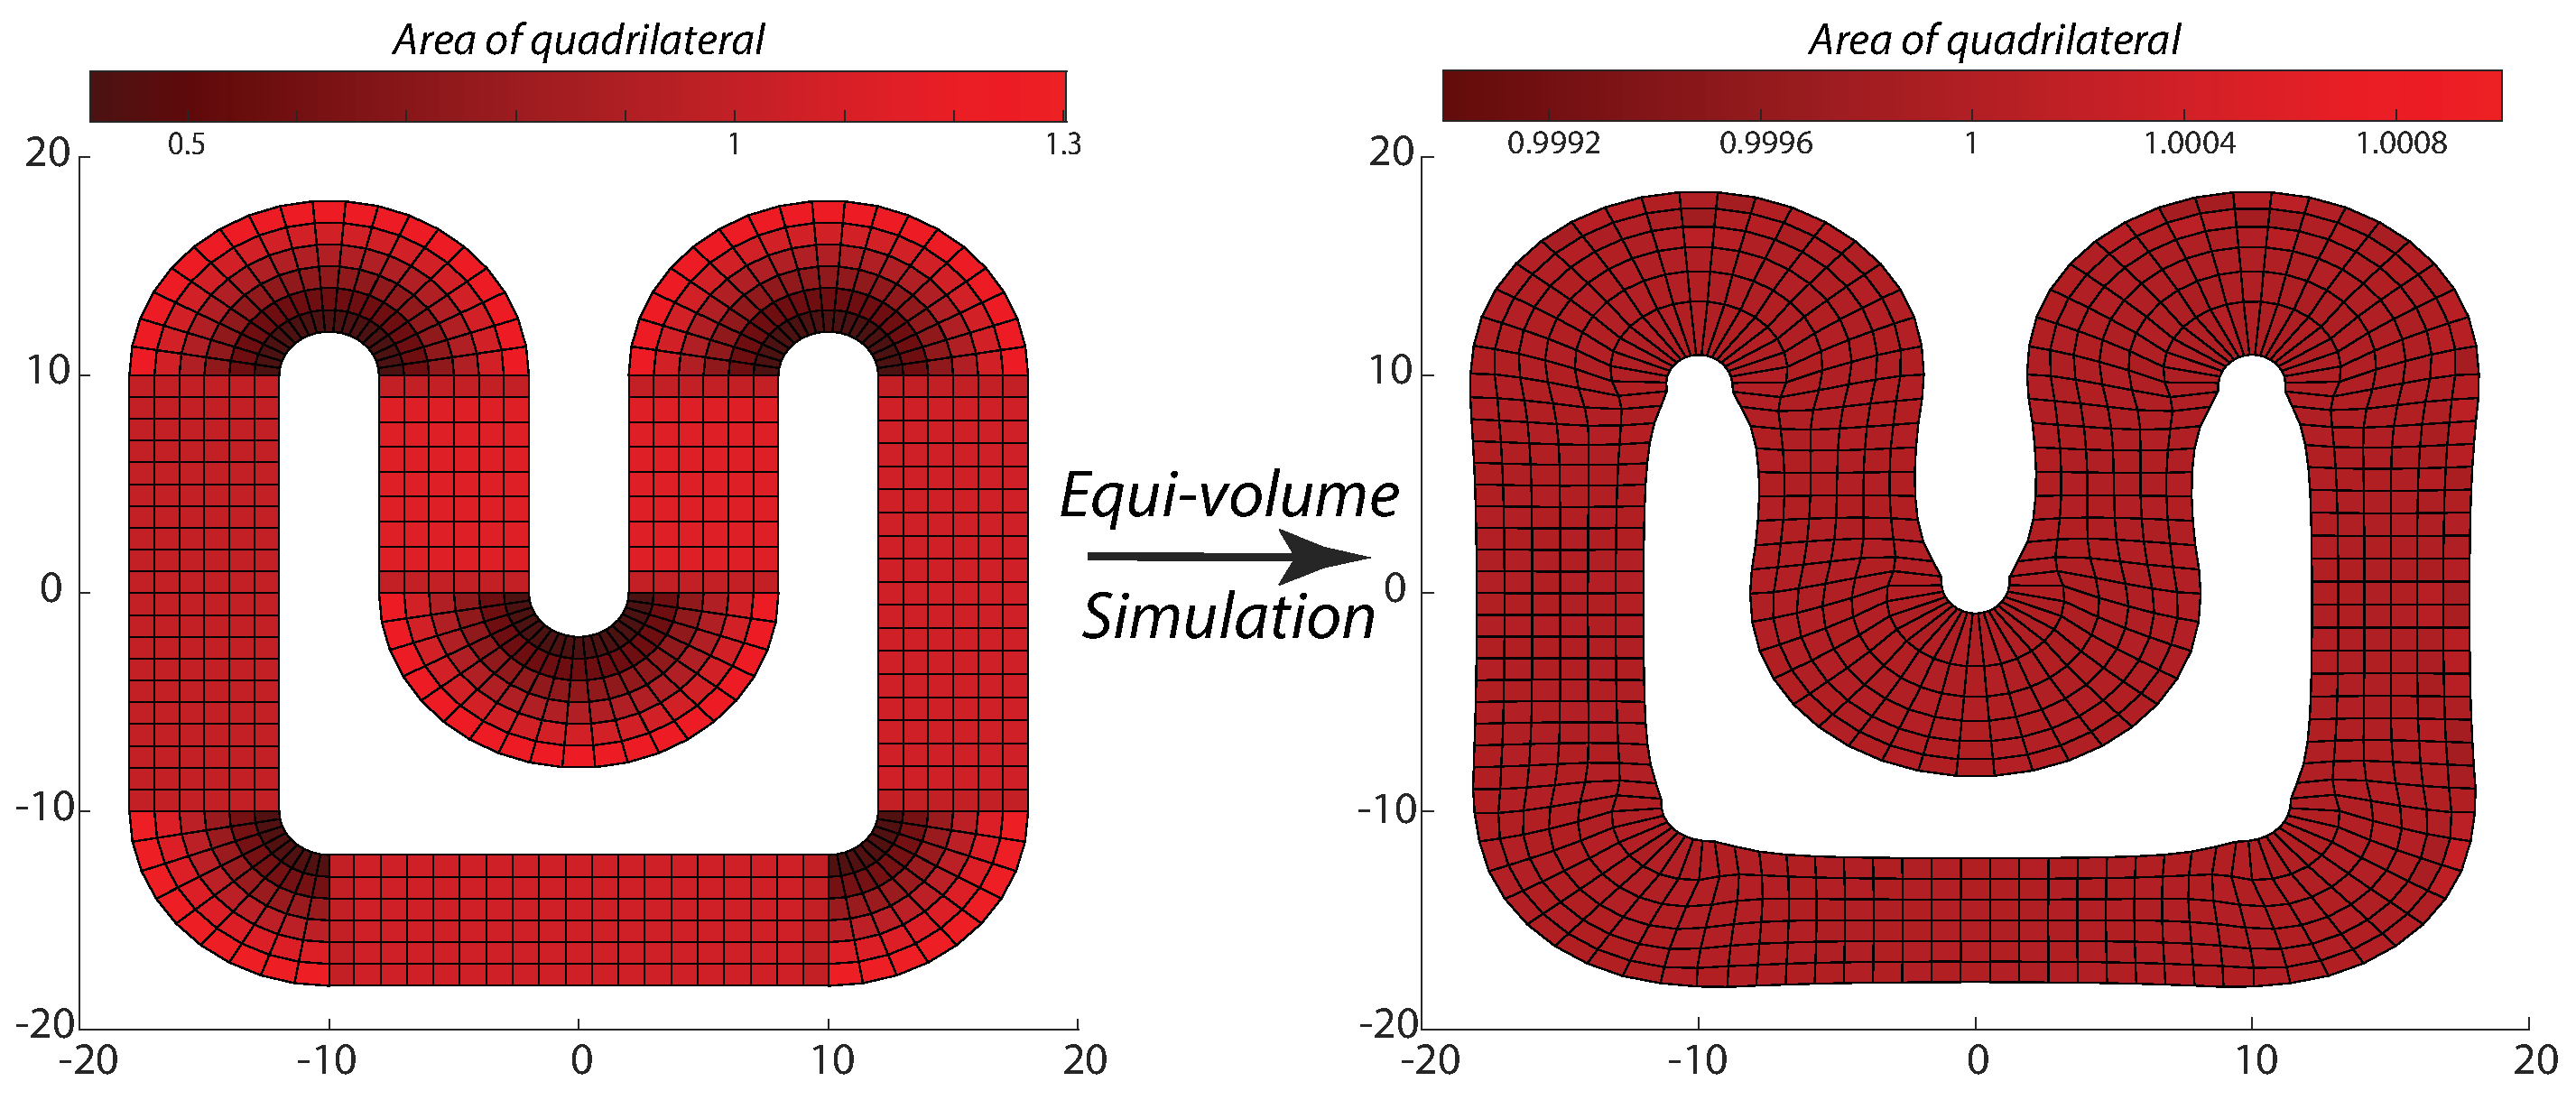
\includegraphics[width=1.\textwidth, clip=true]{./Chapters/03_GLM/./Images/Simulation}
\caption{From an initially equidistant mesh, on the left, we let the points on the mesh rearrange itself in an equivolume manner. The area of a single quadrilateral is indicated by its colour. The resulting mesh, on the right, is rearranged such that all quadrilaterals had unit area ($\pm 10^{-3}$). Note that as a result, the layers start varying in thickness in the inner and outer bends.}
\label{fig:simulation}
\end{figure}

The two-dimensional simulation was first rotated to break alignment with the voxel grid. Next, it was extruded to the third dimension, and resampled to a $64^3$ voxel grid. The simulation covered approximately one voxel per layer. With six layers and an approximate cortical thickness of 3.0 mm \cite{Zilles1990,Fischl2000}, the volume mimicks a resolution of $[0.5$ mm$]^3$. The outer boundaries from the simulation, corresponding to the white matter and pial surfaces, were taken as input for the layering methods. The cortex was divided into six layers and the layering was performed on upsampled data, a factor 2 in each dimension. Treating the simulated layers as a gold standard, the signal leakage between layers can be determined in terms of a spatial point spread function (PSF). The PSF of all methodologies is determined by simulating volumes in which one layer is given the value one; the remainder are set to zero. The extent to which this single layer signal can be retrieved in the correct layer is represented as a PSF. This analysis was performed on a small part of the simulated cortex (ROI shown in Figure~\ref{fig:simulationvolume}) such that positively and negatively curved regions were equally represented. In order to investigate the effect of spatial resolution on the PSF, the simulated data of $[0.5 $mm$]^3$ resolution was downsampled to $[1.0$ mm$]^3$. The same boundaries and the same layering methods and signal extraction procedures were used. No noise was added to the data, so likewise, we did not model any noise covariance in the regression equation and used the ordinary least squares solution.
\begin{figure}[ht]
\centering
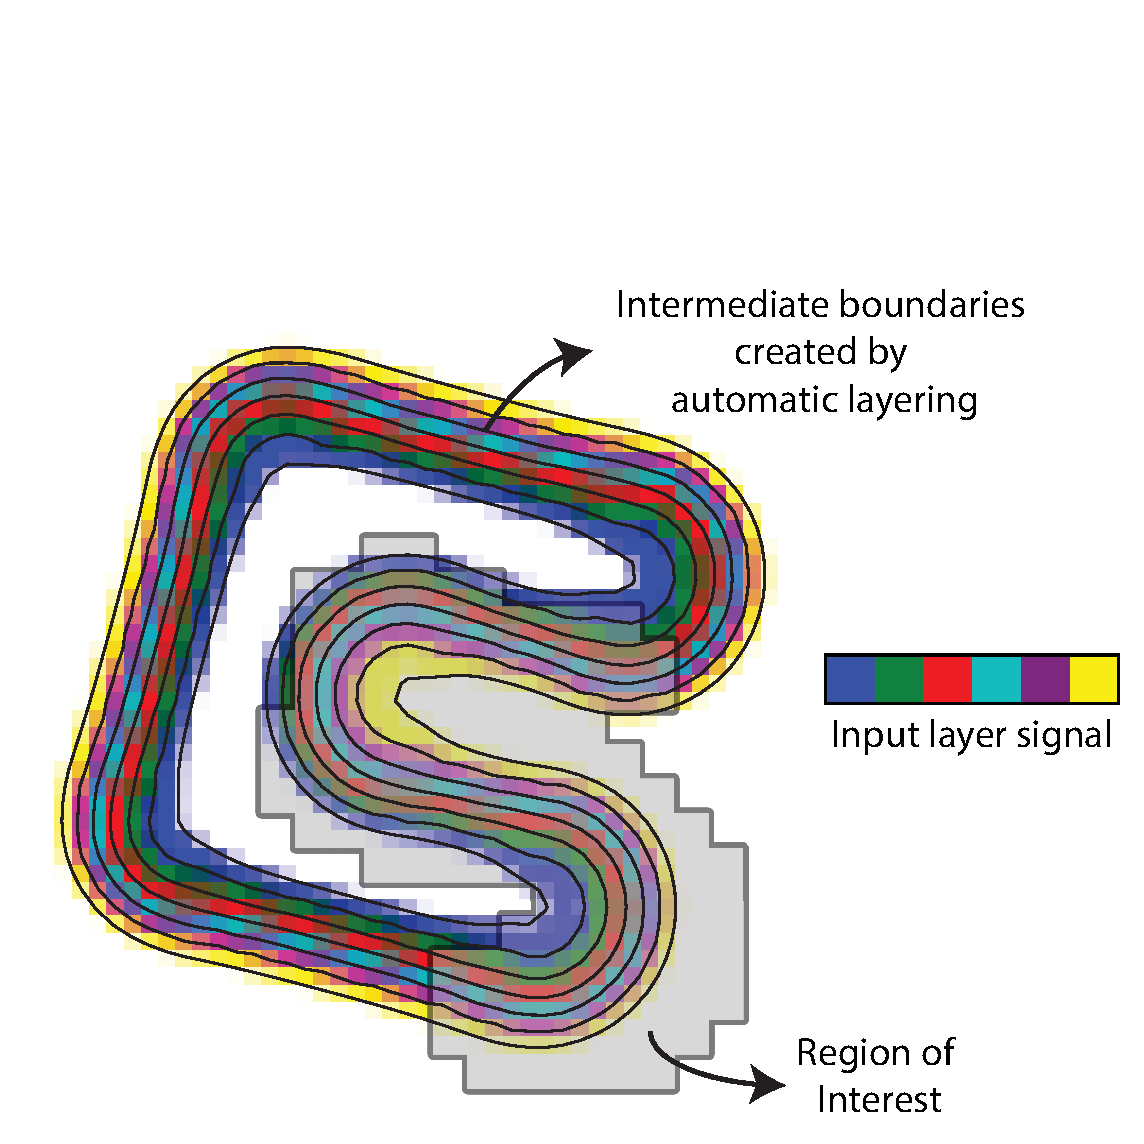
\includegraphics[width=0.7\textwidth, clip=true]{./Chapters/03_GLM/./Images/LayeringSimulation}
\caption{}
\label{fig:simulationvolume}
\end{figure}

\subsection{High-resolution data}
In order to assess the performance of the layer extraction method, we examined a high-resolution post-mortem sample of the visual cortex (V1) of [0.1 mm]$^3$ isotropic resolution. The thickness of this particular region was measured to be between 2 mm and 3 mm. The full experimental setup has been described by Kleinnijenhuis et al. \cite{Kleinnijenhuis2013}. Briefly, prior to MR imaging, samples were fixed (>2 months), soaked in phosphate buffered saline (>72h) and mounted in a syringe with proton-free liquid (\textasciitilde 24h). An MGE (multiple gradient-echo) sequence was used with parameters: TR=3.2 s; 7 echoes; TE1=3.9 ms; echo spacing=5 ms; matrix=250x180; FOV=25x18 mm; TA=612 s. The echoes were averaged and bias field corrected.

The aim was to extract anatomically accurate profiles including the stria of Gennari, a myelinated band of nerve fibres running parallel to the surface that is clearly visible in the image. We wanted to investigate the comparative performance of all methods in a real human cortex, but on clean high resolution data. This way, there was a clear image of the true profile, and sufficient detail that should be revealed in the extracted profile. We classified the grey matter by means of thresholding and manually adapted it to ensure accuracy over the entire region of interest. The pial surface and the white matter surface were created based on these segmentations. From these boundaries, the level set was computed and the layering was performed with 20 equivolume layers. 
\remove{This is equivalent to approximately 1 to 1.5 voxels per layer.}
 Three regions of interest were taken, shown in Fig~\ref{fig:exvivovolume}. They varied in curvature and respectively contained 1757, 924, and 1246 voxels \add{and were 2.07 mm, 2.09 mm, and 1.97 mm thick, so this is equivalent to one layer per voxel}. The results were qualitatively compared. 

\subsection{MP2RAGE data}
Lastly, the method was applied to extract profiles from in-vivo data. We examined the cortical profile of the calcarine sulcus in 11 subjects from a T1-weighted MP2RAGE, acquired with a Siemens 7T scanner, with an isotropic resolution of 1.03 mm$^3$, TR/TE/TI1/TI2 = 5000ms/1.89ms/900ms/3200ms, of the calcarine sulcus. The MP2RAGE was chosen for its homogeneous contrast and sharp transition from white to grey matter, such that the leakage effect to neighbouring layers could be investigated. All scans were processed by FreeSurfer \cite{Dale1999} by means of \texttt{recon-all} and the boundaries generated were used in our layer pipeline. We investigated the effect of number of layers by segmenting the volume into 2, 4, 6, and 8 layers. Additionally, we wanted to test the assumption of correlated noise that we proposed in order to use generalised least squares. We compared four different FWHMs for the noise covariance, 0, 1, 2, and 3 mm, where the 0 mm effectively reduces to an ordinary least squares solution. The region of interest was a small portion of the V1 label from the Destrieux atlas that is automatically generated by FreeSurfer \cite{Fischl2004}. It was trimmed to a small part around the calcarine sulcus, because a fundamental assumption of the GLM is that the layer signal estimates are identical across the entire cortex. This cannot be guaranteed over large patches of cortex, especially because it is known that the myelination throughout the visual cortex is variable, e.g. higher around the calcarine sulcus \cite{Bridge2005}. The number of voxels in the ROI was 2009 $\pm$ 494 $(\mu \pm \sigma)$ and the average thickness was 3.4 mm $\pm$ 0.3 mm $(\mu \pm \sigma)$. An example for a representative subject is shown in Figure~\ref{fig:invivovolume}. The profiles were extracted on the same volume on which the segmentation and cortical reconstruction were performed, so there was no need for image registration.
\begin{figure}[ht]
\centering
\includegraphics[width=0.8\textwidth, clip=true]{./Chapters/03_GLM/./Images/LayeringInVivo}
\caption{The layering (rainbow colours) and the region of interest (pink) for a representative subject. A small portion of an anatomically defined V1 region was taken in order to investigate the cortical profile in the region.}
\label{fig:invivovolume}
\end{figure}

\subsection*{Data Availability}
All source code for the \change{registration algorithm}{spatial GLM} is freely available at \url{https://github.com/TimVanMourik/OpenFmriAnalysis} under the GPL 3.0 license. The respective modules are also available in Porcupine \url{https://timvanmourik.github.io/Porcupine}, a visual pipeline tool that automatically creates custom analysis scripts \cite{VanMourik2017}. All code to generate the images in this paper are available at the Donders Repository \texttt{https://data.donders.ru.nl/login/reviewer-27893111 \\ mzQG7aE5xx2F0zOT1U0qmyVS1hC45dADMqqDWUqn3TU}.

